\documentclass[]{article}

\usepackage{algorithm}
\usepackage{algpseudocode}
\usepackage{url}
\usepackage{tikz}
\usepackage{amsmath,hyperref}
\usepackage{minted}
\usepackage[margin=2.5cm]{geometry}

\usetikzlibrary{positioning}
\usetikzlibrary{shapes.geometric}

\title{\textit{Draft:} Tree Borrows}
\author{y86-dev}

\newcommand{\SHRW}{\texttt{SharedReadWrite} }
\newcommand{\SHRO}{\texttt{SharedReadOnly} }
\newcommand{\SHIR}{\texttt{SharedImmutRead} }
\newcommand{\UNQ}{\texttt{Unique} }
\newcommand{\TPU}{\texttt{Two-Phase-Unique} }

\begin{document}

\maketitle

\textit{This document is a draft. It is still under active development and might contain errors. Many important sections are missing or incomplete.}

\begin{abstract}
This document details an extension of Stacked Borrows. It uses a tree structure instead of the stack to reason
about the soundness of accessing pointers.
\end{abstract}

\section{Overview}
Tree Borrows (TB) is heavily based on the work of \cite{stackedborrows}.
As such, the reader is expected to know the general concepts introduced there.
\subsection{Goals}
TB tries to simplify and improve upon the stack approach by using a tree instead.
Moreover it also aims to solve the issues that arose regarding mutable aliasing \cite{mutable_aliasing}.

We hope to
\begin{itemize}
    \item track interior mutability better.
    \item define when mutable aliasing is allowed.
    \item keep most of the existing behavior.
\end{itemize}

\subsection{Current Issues}
\begin{itemize}
    \item TB does not include untagged pointers, so ptr-int-ptr round trips will always produce pointers with invalid tags. This should not really be a problem, because iirc (y86-dev) non provenance respecting code is going to be UB at some point. This of course poses some problems for code abusing provenance (e.g. XOR linked lists), so maybe we need to add the \texttt{Untagged} pointer-id like SB has today.
    \item TB needs type information at allocation time. I (y86-dev) gave a quick glance at the source code and did find easy access to the type at allocation time. Maybe it is possible to postpone such a type lookup until the first use of the location.
    \item Creating a \texttt{T}, transmuting it to \texttt{UnsafeCell<T>} will not allow \texttt{UnsafeCell}-like access to \texttt{T} (because the original tag of the location will be \UNQ).
\end{itemize}

\subsection{Tags}
TB also tags locations and pointers with so called \textit{tags}.
In addition to the tags from SB, TB introduces new tags: \SHIR and \TPU.
TB does not make use of the \texttt{Disabled} tag, which leaves us with these tags:
\begin{center}
\begin{tabular}{c|c|c}
    & no aliasing & allows aliasing \\
    \hline
    permits writes & \UNQ & \SHRW \\
    \hline
    read only & \SHIR & \SHRO \\
    \hline
    two phase & \TPU
\end{tabular}
\end{center}

Before using a two phase borrow (read/write/retag) remove it from the tree and create a \UNQ/\SHRW with the same id in its place.
This is also a deviation from existing behavior, in SB a retag does not change the two-phase status of a borrow.

\subsubsection{Tag Invariants}

\begin{itemize}
    \item \UNQ: While this pointer tag exists in the borrow tree, all writes to the location need to be carried out by this pointer or any pointer derived from it.
    \item \SHIR: While this pointer tag exists in the borrow tree, the location is not written to.
\end{itemize}
All tags are invalidated (the borrow tree will be cleared/deleted), when their location is \texttt{!Copy} and moved.


\subsubsection{Tag Tree Invariants}
To uphold the invariants mentioned before, these invariants will be enforced upon the tree:

For every
\begin{itemize}
    \item \UNQ:
    \begin{itemize}
        \item other branches contain no \UNQ/\SHRW pointing to the same location.
        \item no \SHIR exists that points to the same location.
        \item no ancestor is a \SHIR
    \end{itemize}
    \item \SHIR: other branches and descendants contain no \UNQ/\SHRW pointing to the same location.
    \item \SHRW: no ancestor is a \SHIR
    \item \TPU: has no descendants
\end{itemize}
And of course it has to be a tree (no cycles and each node has only one outgoing connection).

\subsubsection{Tree Figure Description}
The trees have the following syntax:

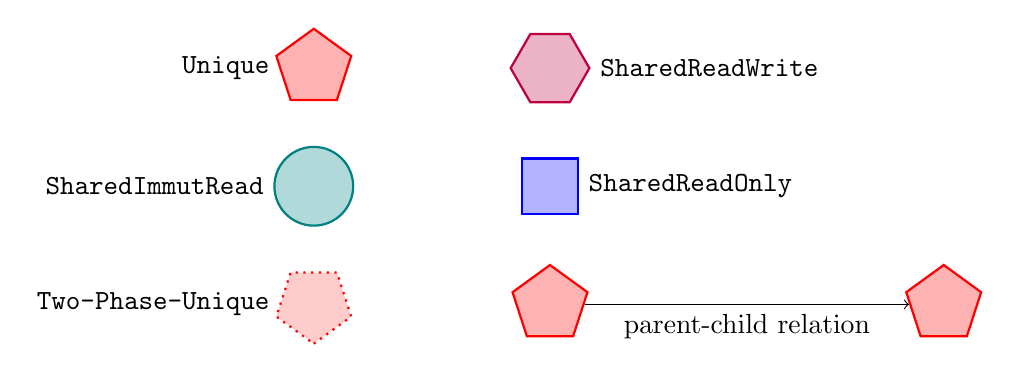
\begin{tikzpicture}[
    unique/.style = {shape = regular polygon, regular polygon sides = 5, draw = red, fill = red!30, thick, minimum size = 1cm, inner sep = 0.1cm},
    tpu/.style = {shape = regular polygon, regular polygon sides = 5, dotted, draw = red, fill = red!20, thick, minimum size = 1cm, inner sep = 0.1cm, shape border rotate =180},
    shrw/.style = {shape = regular polygon, regular polygon sides = 6, thick, draw = purple, fill = purple!30, minimum size = 1cm, inner sep = 0.1cm},
    shro/.style = {shape = regular polygon, regular polygon sides = 4, thick, draw = blue, fill = blue!30, minimum size = 1cm, inner sep = 0.1cm},
    shir/.style = {shape = circle, thick, draw = teal, fill = teal!30, minimum size = 1cm, inner sep = 0.1cm},
    ]
    \node[unique] (A) [label = left:\UNQ] at (0,0) {};
    \node[shir] (B) [label = left:\SHIR] at (0, -1.5) {};
    \node[shro] (C) [label = right:\SHRO] at (3, -1.5) {};
    \node[shrw] (E) [label = right:\SHRW] at (3, 0) {};
    \node[unique] (F) [label = right:\texttt{}] at (3, -3) {};
    \node[unique] (G) [label = right:\texttt{}] at (8, -3) {};
    \node[tpu] (H) [label = left:\TPU] at (0,-3) {};
    
    \path[->](F) edge node[below] {parent-child relation} (G);
\end{tikzpicture}

\subsubsection{Examples of Valid Trees}

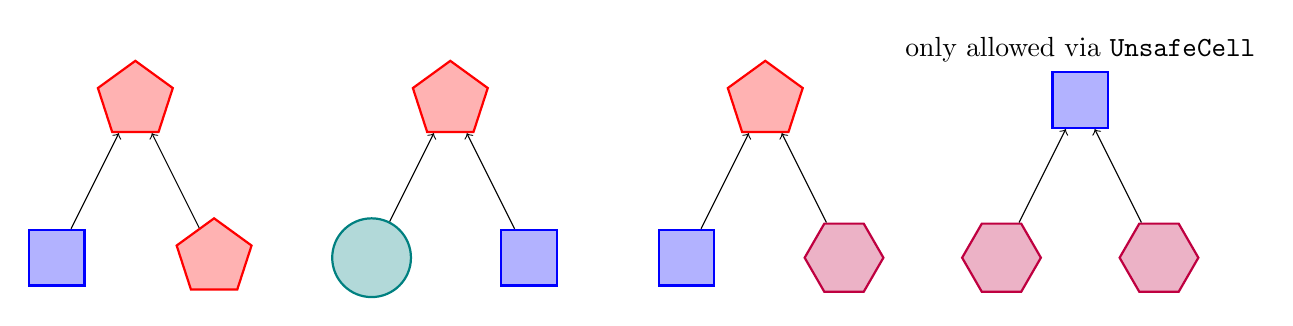
\begin{tikzpicture}[
    unique/.style = {shape = regular polygon, regular polygon sides = 5, draw = red, fill = red!30, thick, minimum size = 1cm, inner sep = 0.1cm},
    shrw/.style = {shape = regular polygon, regular polygon sides = 6, thick, draw = purple, fill = purple!30, minimum size = 1cm, inner sep = 0.1cm},
    shro/.style = {shape = regular polygon, regular polygon sides = 4, thick, draw = blue, fill = blue!30, minimum size = 1cm, inner sep = 0.1cm},
    shir/.style = {shape = circle, thick, draw = teal, fill = teal!30, minimum size = 1cm, inner sep = 0.1cm},
    ]
    \node[unique] (A1) at (0, 0) {};
    \node[unique] (B1) at (1, -2) {};
    \node[shro] (C1) at (-1, -2) {};
    
    \path[->](B1) edge node[left] {} (A1);
    \path[->](C1) edge node[left] {} (A1);
    
    \node[unique] (A2) at (4, 0) {};
    \node[shro] (B2) at (5, -2) {};
    \node[shir] (C2) at (3, -2) {};
    
    \path[->](B2) edge node[left] {} (A2);
    \path[->](C2) edge node[left] {} (A2);
    
    \node[unique] (A3) at (8, 0) {};
    \node[shrw] (B3) at (9, -2) {};
    \node[shro] (C3) at (7, -2) {};
    
    \path[->](B3) edge node[left] {} (A3);
    \path[->](C3) edge node[left] {} (A3);
    
    \node[shro] (A4) [label = above:only allowed via \texttt{UnsafeCell}] at (12, 0) {};
    \node[shrw] (B4) at (13, -2) {};
    \node[shrw] (C4) at (11, -2) {};
    
    \path[->](B4) edge node[left] {} (A4);
    \path[->](C4) edge node[left] {} (A4);
\end{tikzpicture}

\subsubsection{Examples of Invalid Trees}

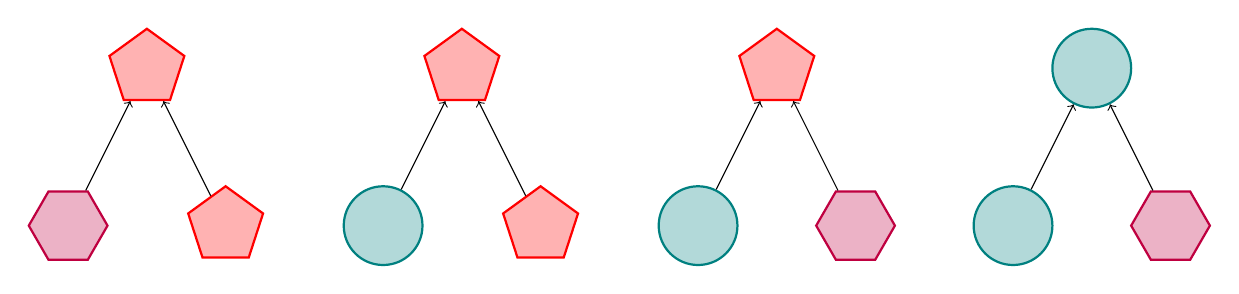
\begin{tikzpicture}[
    unique/.style = {shape = regular polygon, regular polygon sides = 5, draw = red, fill = red!30, thick, minimum size = 1cm, inner sep = 0.1cm},
    shrw/.style = {shape = regular polygon, regular polygon sides = 6, thick, draw = purple, fill = purple!30, minimum size = 1cm, inner sep = 0.1cm},
    shro/.style = {shape = regular polygon, regular polygon sides = 4, thick, draw = blue, fill = blue!30, minimum size = 1cm, inner sep = 0.1cm},
    shir/.style = {shape = circle, thick, draw = teal, fill = teal!30, minimum size = 1cm, inner sep = 0.1cm},
    ]
    \node[unique] (A1) at (0, 0) {};
    \node[unique] (B1) at (1, -2) {};
    \node[shrw] (C1) at (-1, -2) {};
    
    \path[->](B1) edge node[left] {} (A1);
    \path[->](C1) edge node[left] {} (A1);
    
    \node[unique] (A2) at (4, 0) {};
    \node[unique] (B2) at (5, -2) {};
    \node[shir] (C2) at (3, -2) {};
    
    \path[->](B2) edge node[left] {} (A2);
    \path[->](C2) edge node[left] {} (A2);
    
    \node[unique] (A3) at (8, 0) {};
    \node[shrw] (B3) at (9, -2) {};
    \node[shir] (C3) at (7, -2) {};
    
    \path[->](B3) edge node[left] {} (A3);
    \path[->](C3) edge node[left] {} (A3);
    
    \node[shir] (A4) at (12, 0) {};
    \node[shrw] (B4) at (13, -2) {};
    \node[shir] (C4) at (11, -2) {};
    
    \path[->](B4) edge node[left] {} (A4);
    \path[->](C4) edge node[left] {} (A4);
\end{tikzpicture}

\subsection{Tree Operations}
\subsubsection{Allocating}
Each location will be tracked by one tree. When creating an allocation the root node of the tree is created. Its tag is
determined by the nature of the allocation\footnote{What about \texttt{Box} and other smart pointers? We also need to track allocations done by the allocator. They should receive the same treatment as \texttt{let mut x: T = ...;}}:\\
When \texttt{T} is not \texttt{UnsafeCell}/\texttt{UnsafeAliasCell}:
\begin{itemize}
    \item \texttt{let x: T = ...;} $\implies$ \SHIR
    \item \texttt{let mut x: T = ...;} $\implies$ \UNQ
    \item \texttt{static x: T = ...;} $\implies$ \SHIR
    \item \texttt{static mut x: T = ...;} $\implies$ \SHRW
\end{itemize}
\texttt{UnsafeCell}:
\begin{itemize}
\item \texttt{let x: UnsafeCell<T> = ...;} $\implies$ \SHRO
\item \texttt{let mut x: UnsafeCell<T> = ...;} $\implies$ \SHRO
\item \texttt{static x: UnsafeCell<T> = ...;} $\implies$ \SHRO
\item \texttt{static mut x: UnsafeCell<T> = ...;} $\implies$ \SHRW
\end{itemize}
\texttt{UnsafeAliasCell}:
\begin{itemize}
\item \texttt{let x: UnsafeAliasCell<T> = ...;} $\implies$ \SHRW
\item \texttt{let mut x: UnsafeAliasCell<T> = ...;} $\implies$ \SHRW
\item \texttt{static x: UnsafeAliasCell<T> = ...;} $\implies$ \SHRW
\item \texttt{static mut x: UnsafeAliasCell<T> = ...;} $\implies$ \SHRW
\end{itemize}
When \texttt{T} contains an \texttt{UnsafeCell}/\texttt{UnsafeAliasCell} then we allocate each value contained separately,
allocate memory for the type as if it did not contain any \texttt{Cells} and then move each field to its respective position.
When moving the contents of a location, we also move the tag to the new location.
This results in us finely tracking values stored in \texttt{UnsafeCell}/\texttt{UnsafeAliasCell}
even within enums and unions \footnote{I (y86-dev) have no idea if the type can be known at allocation time in miri. I glanced at the source code and was not able to find easy
    access to the type information at the creation site of the \texttt{Stacks} struct in current SB.}.

\subsubsection{Read Access}

When reading we need to ensure that the tag still exists. Additional care needs to be taken, to ensure our variants are still upheld.

Reading a pointer with tag \UNQ will change all derived \UNQ $\mapsto$ \SHIR and all derived \SHRW $\mapsto$ \SHRO. This ensures that two reads of the same \UNQ pointer will result in the same value, if that pointer is never used to write in between (deriving a new pointer with write permission counts as a write access to the original pointer).

Reading a pointer with a different tag does not require any modification of the tree. Only a check for existence of the pointer tag.

\subsubsection{Write Access}

Writing to a pointer with tag \UNQ will remove all derived \UNQ, \SHIR and \TPU pointers, inheriting any of their \SHRO children. All derived \SHRW will be turned into \SHRO. This re-asserts the uniqueness of the pointer (removing all derived aliasing pointers/turning them into read only) and prevents future reads using a \SHIR (because that pointer would then observe a written-to value) and prevents future activation of any \TPU.

Writing to a pointer with tag \SHRW does not require any any modification of the tree. Only a check for existence of the pointer tag.

\subsubsection{New Pointer Creation}
When casting a reference to a raw pointer (\UNQ / \SHIR $\mapsto$ \SHRW / \SHRO, or \UNQ $\mapsto$ \TPU)  or reborrowing a reference, treat it the same as a write/read access of that pointer.

When deriving a pointer with \UNQ / \SHIR tag from a pointer with \SHRW / \SHRO tag, we might need to modify the tree:
\begin{itemize}
    \item \SHRW $\mapsto$ \UNQ:
    \begin{enumerate}
        \item check if the pointer tag exists
        \item remove all descendants with \UNQ, \SHRW, \SHIR, \TPU tag and inherit their children.
        \item recurs the tree upwards to the root, exploring any side branches (all branches where the \SHRW is not a descendant) and remove all descendants with \UNQ, \SHRW, \SHIR, \TPU tag and inherit their children to the branching ancestor.
    \end{enumerate}
    \item \texttt{*} $\mapsto$ \SHIR
    \begin{enumerate}
        \item check if the pointer tag exists
        \item replace all \UNQ/ \SHRW descendants with \SHIR/\SHRO
        \item recurs the tree upwards to the root, exploring any side branches (all branches where the \texttt{*} is not a descendant) and replace all \UNQ/ \SHRW descendants with \SHIR/ \SHRO.
    \end{enumerate}
\end{itemize}

\noindent There are only three legal ways to turn \texttt{*const T} into \texttt{*mut T}:
\begin{itemize}
    \item the \texttt{get()} function of \texttt{UnsafeCell}
    \item the \texttt{get()} function of \texttt{UnsafeAliasCell}
    \item pointer casting \texttt{*const T} to \texttt{*mut T}, if the original raw pointer that was created was \texttt{*mut T} (so round tripping \texttt{*mut T} $\mapsto$ \texttt{*const T} $\mapsto$\texttt{*mut T} is allowed).
\end{itemize}

\subsubsection{Moving}

When moving a value, the trees for the locations will be removed. This prevents read/write after move.

\subsection{Comparison With the Stack}
\subsubsection{\UNQ and \SHIR}
When only \SHIR and \UNQ are used, the tree behaves exactly as the stack would.
When only using \UNQ, there can only exist one branch containing \UNQ at any one time. Creating a new branch will either extend or remove the previous branch.

When also dealing with \SHIR, the tree may ``freeze'' when a \SHIR is created, turning all \UNQ that are below the parent pointer into \SHIR's as well. When a \UNQ above the parent is used (all the \UNQ's above the parent will still remain) then all pointers below it will be removed, leaving us again with a single branch of \UNQ's.

This is almost exactly the same behavior as the stack, only giving more information about the relation of two \SHIR's (in the stack you cannot know if they are derived from each other or from a different pointer further down the stack).

\subsubsection{\SHRO and \SHRW}
When creating \SHRO and \SHRW the tree will also branch (like when using \newline\SHIR), but this time one can write using \SHRW pointers and observe locations that are written to with \SHRO.

The invariants of \SHIR and \UNQ are still upheld, so when using one, \SHRW will be transformed into \SHRO and further writes will be denied. \SHRO will not be disturbed by anything (except location moves of \texttt{!Copy} data) and thus one is allowed to read the memory even if there exist any other pointers.

The Stack has to add some non-stack operations to support these pointers, inserting below already added elements and replacing \UNQ with \texttt{Disabled} to still allow access via \SHRW when the parent \UNQ is invalidated.

\subsubsection{\TPU}
A \TPU behaves almost exactly as a \SHIR, when a \SHRW or \UNQ is created, any \TPU is removed and will not allow future activation. On activation (TB also activates on retag) it is replaced by a \UNQ and counts as a write-use of the parent pointer, thus invalidating any aliasing \SHIR's.

SB maps two-phase borrows to \SHRW, requiring additional information from MIR when a two-phase borrow is activated.\footnote{Needs verification}

\subsection{Protectors}
Protectors are still needed in TB, as they solve the same problem that is also present in SB.

\section{Rationale}
\textit{this section does not yet contain a formal proof.}
\\

\subsection{Examples from the SB paper}
\subsubsection{Evil RefCell}
{\small
\begin{minted}{rust}
fn evil_ref_cell (shared : &RefCell<i32>, mutable : &mut i32) {
    retag [fn] shared; retag [fn] mutable;
    let more_shared = &*shared;
    *mutable = 23;
}
fn main() {
    let cell = RefCell::new(42);
    evil_ref_cell(&cell, &mut *cell.borrow_mut().unwrap());
}
\end{minted}
}
This is the tree right before \texttt{more\_shared} gets created:


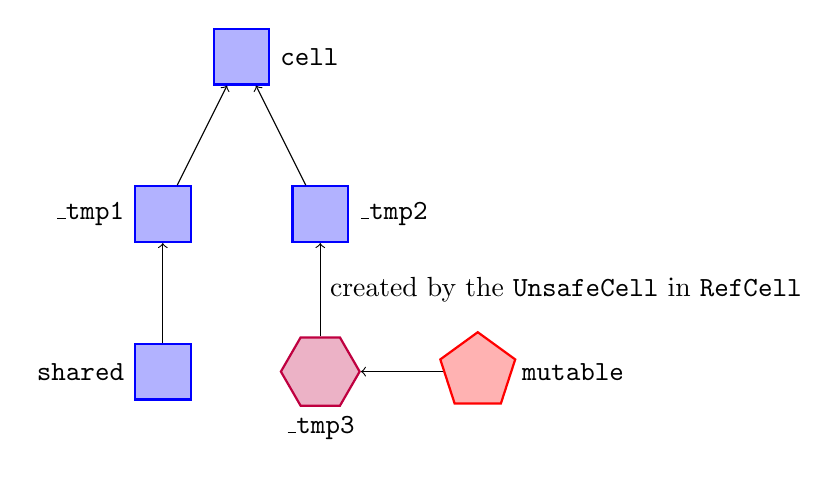
\begin{tikzpicture}[
        unique/.style = {shape = regular polygon, regular polygon sides = 5, draw = red, fill = red!30, thick, minimum size = 1cm, inner sep = 0.1cm},
        shrw/.style = {shape = regular polygon, regular polygon sides = 6, thick, draw = purple, fill = purple!30, minimum size = 1cm, inner sep = 0.1cm},
        shro/.style = {shape = regular polygon, regular polygon sides = 4, thick, draw = blue, fill = blue!30, minimum size = 1cm, inner sep = 0.1cm},
        shir/.style = {shape = circle, thick, draw = teal, fill = teal!30, minimum size = 1cm, inner sep = 0.1cm},
    ]
    \node[shro] (A) [label = right:\texttt{cell}] at (0,0) {};
    \node[shro] (B) [label = left:\texttt{\_tmp1}] at (-1, -2) {};
    \node[shro] (C) [label = right:\texttt{\_tmp2}] at (1, -2) {};
    \node[shro] (D) [label = left:\texttt{shared}] at (-1, -4) {};
    \node[shrw] (E) [label = below:\texttt{\_tmp3}] at (1, -4) {};
    \node[unique] (F) [label = right:\texttt{mutable}] at (3, -4) {};
    
    \path[->](B) edge node[left] {} (A);
    \path[->](C) edge node[left] {} (A);
    \path[->](D) edge node[left] {} (B);
    \path[->](E) edge node[right] {created by the \texttt{UnsafeCell} in \texttt{RefCell}} (C);
    \path[->](F) edge node[left] {} (E);
\end{tikzpicture}

When \texttt{more\_shared} gets created, we reborrow the \SHRO, which specifically allows mutation via aliasing pointers.
The new tree just has an extra node with \texttt{shared} as the parent:


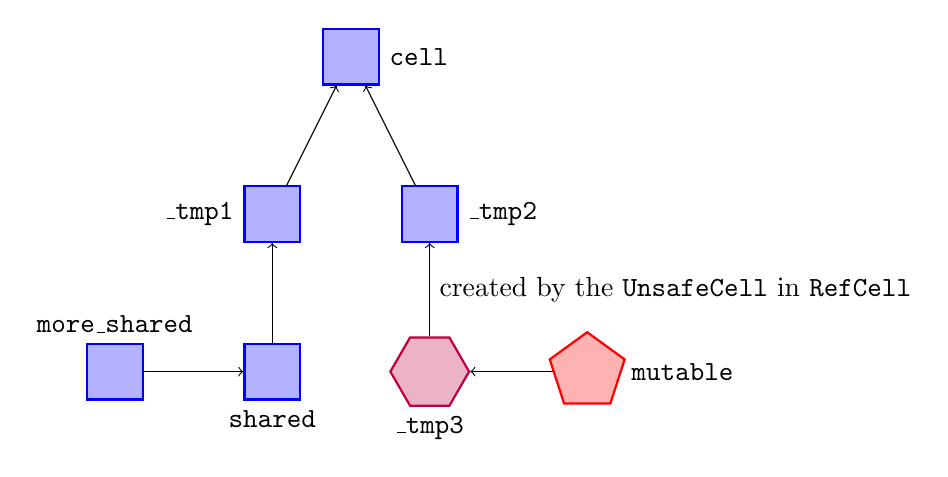
\begin{tikzpicture}[
    unique/.style = {shape = regular polygon, regular polygon sides = 5, draw = red, fill = red!30, thick, minimum size = 1cm, inner sep = 0.1cm},
    shrw/.style = {shape = regular polygon, regular polygon sides = 6, thick, draw = purple, fill = purple!30, minimum size = 1cm, inner sep = 0.1cm},
    shro/.style = {shape = regular polygon, regular polygon sides = 4, thick, draw = blue, fill = blue!30, minimum size = 1cm, inner sep = 0.1cm},
    shir/.style = {shape = circle, thick, draw = teal, fill = teal!30, minimum size = 1cm, inner sep = 0.1cm},
    ]
    \node[shro] (A) [label = right:\texttt{cell}] at (0,0) {};
    \node[shro] (B) [label = left:\texttt{\_tmp1}] at (-1, -2) {};
    \node[shro] (C) [label = right:\texttt{\_tmp2}] at (1, -2) {};
    \node[shro] (D) [label = below:\texttt{shared}] at (-1, -4) {};
    \node[shrw] (E) [label = below:\texttt{\_tmp3}] at (1, -4) {};
    \node[unique] (F) [label = right:\texttt{mutable}] at (3, -4) {};
    \node[shro] (G) [label = above:\texttt{more\_shared}] at (-3, -4) {};
    
    \path[->](B) edge node[left] {} (A);
    \path[->](C) edge node[left] {} (A);
    \path[->](D) edge node[left] {} (B);
    \path[->](E) edge node[right] {created by the \texttt{UnsafeCell} in \texttt{RefCell}} (C);
    \path[->](F) edge node[left] {} (E);
    \path[->](G) edge node[left] {} (D);
\end{tikzpicture}

\subsubsection{Bad Raw Pointer Pattern}
{\small
\begin{minted}{rust}
fn make_raw (y: &mut i32) -> * mut i32 { retag [fn] y; y as *mut i32 }

fn bad_pattern (x: &mut i32) {
    retag [fn] x;
    let raw_ptr = make_raw(x);
    // Point of interest 1
    let val1 = *x;
    // Point of interest 2
    let val2 = unsafe { *raw_ptr };
}
\end{minted}
}

After PoI 1 the borrow tree will look like this:


\begin{tikzpicture}[
    unique/.style = {shape = regular polygon, regular polygon sides = 5, draw = red, fill = red!30, thick, minimum size = 1cm, inner sep = 0.1cm},
    shrw/.style = {shape = regular polygon, regular polygon sides = 6, thick, draw = purple, fill = purple!30, minimum size = 1cm, inner sep = 0.1cm},
    shro/.style = {shape = regular polygon, regular polygon sides = 4, thick, draw = blue, fill = blue!30, minimum size = 1cm, inner sep = 0.1cm},
    shir/.style = {shape = circle, thick, draw = teal, fill = teal!30, minimum size = 1cm, inner sep = 0.1cm},
    ]
    \node (origin) [left = of A]{$\dots$};
    \node[unique] (A) {x};
    \node[unique] (B) [right = of A, label = below:\texttt{\_tmp1}] {};
    \node[unique] (C) [right = of B] {y};
    \node[shrw] (D) [right = of C, label = below:\texttt{raw\_ptr}] {};
    
    \path[->](A) edge node[left] {} (origin);
    \path[->](B) edge node[left] {} (A);
    \path[->](C) edge node[left] {} (B);
    \path[->](D) edge node[left] {} (C);
\end{tikzpicture}

We then access \texttt{x} for reading, thus revoking write access from all descendants. The tree now looks like this (at PoI 2):

\begin{tikzpicture}[
    unique/.style = {shape = regular polygon, regular polygon sides = 5, draw = red, fill = red!30, thick, minimum size = 1cm, inner sep = 0.1cm},
    shrw/.style = {shape = regular polygon, regular polygon sides = 6, thick, draw = purple, fill = purple!30, minimum size = 1cm, inner sep = 0.1cm},
    shro/.style = {shape = regular polygon, regular polygon sides = 4, thick, draw = blue, fill = blue!30, minimum size = 1cm, inner sep = 0.1cm},
    shir/.style = {shape = circle, thick, draw = teal, fill = teal!30, minimum size = 1cm, inner sep = 0.1cm},
    ]
    \node (origin) [left = of A]{$\dots$};
    \node[unique] (A) {x};
    \node[shir] (B) [right = of A, label = below:\texttt{\_tmp1}] {};
    \node[shir] (C) [right = of B] {y};
    \node[shro] (D) [right = of C, label = below:\texttt{raw\_ptr}] {};
    
    \path[->](A) edge node[left] {} (origin);
    \path[->](B) edge node[left] {} (A);
    \path[->](C) edge node[left] {} (B);
    \path[->](D) edge node[left] {} (C);
\end{tikzpicture}

When we now try to read from \texttt{raw\_ptr}, then this is still allowed, because it still exists in the tree.

\subsection{More Examples}
\subsubsection{Mutable Pointer Reborrow}
{\small
\begin{minted}{rust}
fn main() { unsafe {
    let mut x = 0;
    let ptr1 = &mut x as *mut i32;
    // PoI 1
    let ptr2 = &mut x as *mut i32;
    // PoI 2
    *ptr1 = 42;
//  ^^^^^ error: tag not in the borrow tree
    *ptr2 = 60;
} }
\end{minted}
}

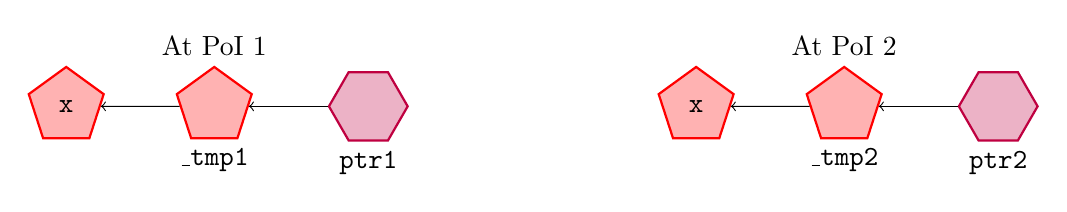
\begin{tikzpicture}[
unique/.style = {shape = regular polygon, regular polygon sides = 5, draw = red, fill = red!30, thick, minimum size = 1cm, inner sep = 0.1cm},
shrw/.style = {shape = regular polygon, regular polygon sides = 6, thick, draw = purple, fill = purple!30, minimum size = 1cm, inner sep = 0.1cm},
shro/.style = {shape = regular polygon, regular polygon sides = 4, thick, draw = blue, fill = blue!30, minimum size = 1cm, inner sep = 0.1cm},
shir/.style = {shape = circle, thick, draw = teal, fill = teal!30, minimum size = 1cm, inner sep = 0.1cm},
]
\node[unique] (A) at (0, 0) {\texttt{x}};
\node[unique] (B) [right = of A, label = below:\texttt{\_tmp1}, label = above:At PoI 1] {};
\node[shrw] (C) [right = of B, label = below:\texttt{ptr1}] {};

\path[->](B) edge node[left] {} (A);
\path[->](C) edge node[left] {} (B);

\node[unique] (A1) at (8, 0) {\texttt{x}};
\node[unique] (B1) [right = of A1, label = below:\texttt{\_tmp2}, label = above:At PoI 2] {};
\node[shrw] (C1) [right = of B1, label = below:\texttt{ptr2}] {};

\path[->](B1) edge node[left] {} (A1);
\path[->](C1) edge node[left] {} (B1);
\end{tikzpicture}

\subsubsection{SharedReadWrite Reborrow}
Creating raw pointers directly without temporary mutable references is ok:

{\small
\begin{minted}{rust}
fn main() { unsafe {
    let mut x = 0;
    let ptr1 = addr_of_mut!(x);
    // PoI 1
    let ptr2 = addr_of_mut!(x);
    // PoI 2
    *ptr1 = 42;
    *ptr2 = 60;
} }
\end{minted}
}

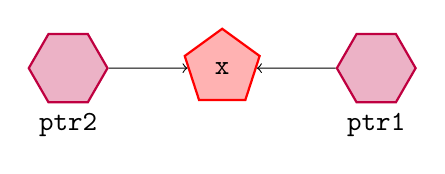
\begin{tikzpicture}[
unique/.style = {shape = regular polygon, regular polygon sides = 5, draw = red, fill = red!30, thick, minimum size = 1cm, inner sep = 0.1cm},
shrw/.style = {shape = regular polygon, regular polygon sides = 6, thick, draw = purple, fill = purple!30, minimum size = 1cm, inner sep = 0.1cm},
shro/.style = {shape = regular polygon, regular polygon sides = 4, thick, draw = blue, fill = blue!30, minimum size = 1cm, inner sep = 0.1cm},
shir/.style = {shape = circle, thick, draw = teal, fill = teal!30, minimum size = 1cm, inner sep = 0.1cm},
]
\node[unique] (A) at (0, 0) {\texttt{x}};
\node[shrw] (C) [right = of A, label = below:\texttt{ptr1}] {};

\path[->](C) edge node[left] {} (A);

\node[shrw] (C1) [left = of A, label = below:\texttt{ptr2}] {};

\path[->](C1) edge node[left] {} (A);
\end{tikzpicture}

\section{Unresolved Patterns}
This section goes over some examples which exhibit not yet finalized behavior.
\subsection{Deviations From SB/Miri}
\subsubsection{Allow reading from \texttt{*mut T} after writes using the parent \texttt{\&mut T}}
TB does not consider this as UB, but miri does:
{\small
\begin{minted}{rust}
fn main() { unsafe {
    let mut x_location = 0;      
    let x = &mut x;
    let ptr = &mut *x as *mut i32;
    // PoI 1
    *x += 42;
    // PoI 2
    println!("{:?}", *ptr);
    //               ^^^^ miri errors here: trying to reborrow <untagged> for SharedReadOnly
    // permission at alloc1283[0x0], but that tag does not exist in the borrow stack for this location
} }
\end{minted}
}

Under TB the tree looks like this at Poi 1:

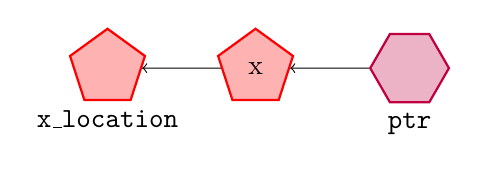
\begin{tikzpicture}[
    unique/.style = {shape = regular polygon, regular polygon sides = 5, draw = red, fill = red!30, thick, minimum size = 1cm, inner sep = 0.1cm},
    shrw/.style = {shape = regular polygon, regular polygon sides = 6, thick, draw = purple, fill = purple!30, minimum size = 1cm, inner sep = 0.1cm},
    shro/.style = {shape = regular polygon, regular polygon sides = 4, thick, draw = blue, fill = blue!30, minimum size = 1cm, inner sep = 0.1cm},
    shir/.style = {shape = circle, thick, draw = teal, fill = teal!30, minimum size = 1cm, inner sep = 0.1cm},
    ]
    \node[unique] (A) [label = below:\texttt{x\_location}] {};
    \node[unique] (B) [right = of A, label = below:\texttt{}] {x};
    \node[shrw] (C) [right = of B, label = below:\texttt{ptr}] {};
    
    \path[->](B) edge node[left] {} (A);
    \path[->](C) edge node[left] {} (B);
\end{tikzpicture}

At Poi 2, the write to \texttt{x} has turned the \SHRW into a \SHRO:

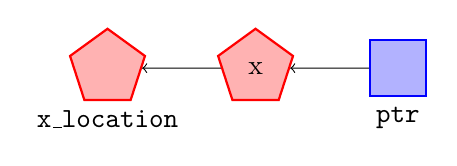
\begin{tikzpicture}[
unique/.style = {shape = regular polygon, regular polygon sides = 5, draw = red, fill = red!30, thick, minimum size = 1cm, inner sep = 0.1cm},
shrw/.style = {shape = regular polygon, regular polygon sides = 6, thick, draw = purple, fill = purple!30, minimum size = 1cm, inner sep = 0.1cm},
shro/.style = {shape = regular polygon, regular polygon sides = 4, thick, draw = blue, fill = blue!30, minimum size = 1cm, inner sep = 0.1cm},
shir/.style = {shape = circle, thick, draw = teal, fill = teal!30, minimum size = 1cm, inner sep = 0.1cm},
]
\node[unique] (A) [label = below:\texttt{x\_location}] {};
\node[unique] (B) [right = of A, label = below:\texttt{}] {x};
\node[shro] (C) [right = of B, label = below:\texttt{ptr}] {};

\path[->](B) edge node[left] {} (A);
\path[->](C) edge node[left] {} (B);
\end{tikzpicture}

This would then allow reading from that pointer.


\textbf{In favor of this behavior:}
\begin{itemize}
    \item natural and consistent behavior of aliasing pointers (if you were to cast ptr to \texttt{*const i32} then this would also allow later reads).
    \item enforces the uniqueness of the write ability of \texttt{\&mut}
\end{itemize}

\textbf{Against this behavior:}
\begin{itemize}
    \item deviating from current SB and miri behavior.
    \item disallows this pattern (SB/miri is ok with this):
{\small
\begin{minted}{rust}
fn main() { unsafe {
    let mut x = 0;  
    let x = &mut x;
    let ptr1 = &mut *x as *mut i32;
    let ptr2 = ptr1;
    *ptr1 += 20;
    *ptr2 += 1;
    println!("{:?}", *x);
    //               ^^ TB note: this read to an Unique pointer revokes
    //                           the write access of all derived pointers.
    *ptr1 += 1;
//  ^^^^^ TB error: tried to write using a SharedReadOnly pointer derived from x.
    *ptr2 += 20;
    println!("{:?}", *x);
} }
\end{minted}
}
\end{itemize}

\subsubsection{Use/Write after move}
TB considers this UB, but miri does not:
{\small
\begin{minted}{rust}
fn main() { unsafe {
    let mut x = "Hello world!".to_owned();
    println!("addr of x: {:p}", &x);
    let ptr = &mut x as *mut String;
    let y = x;
    println!("addr of y: {:p}", &y);
    println!("ptr points to {ptr:p}");
    println!("{}", *ptr);
    //             ^^^^ TB error: tried to read using SharedReadWrite <tag>,
    //                            but that tag points to a location without a borrow tree.
} }
\end{minted}
}


\textbf{In favor of this behavior:}
\begin{itemize}
    \item behavior reflecting the borrow checker.
    \item allow future optimization (e.g. reuse of stack memory)
\end{itemize}

\textbf{Against this behavior:}
\begin{itemize}
    \item deviating from current SB and miri behavior.
\end{itemize}

\newpage

\section{Open Questions}
While writing this document we came across the following questions and did not find an immediate answer to them:
\begin{itemize}
    \item Is it allowed to create multiple two-phase borrows to the same location at the same time and then only activate one?
\end{itemize}

\bibliographystyle{plain}
\bibliography{treeborrows}

\end{document}
